\section{Sezione Tecnico}
\label{sec:sezTecnico}

\subsection*{Avviso}
Per accedere alle funzionalità del Tecnico è necessario effettuare il login con successo. Le credenziali di accesso sono:
\begin{itemize}
    \item \textbf{Nome utente} (username): admin;
    \item \textbf{Password}: admin. 
\end{itemize}

\subsection{Autenticazione}
Nella sezione superiore destra dell'interfaccia, cliccando sull'icona di login 
\includegraphics[height=1.2em]{assets/user_icon.png}, l'Utente può inserire le credenziali per sbloccare le funzionalità del Tecnico.
\begin{figure}[H]
  \centering
  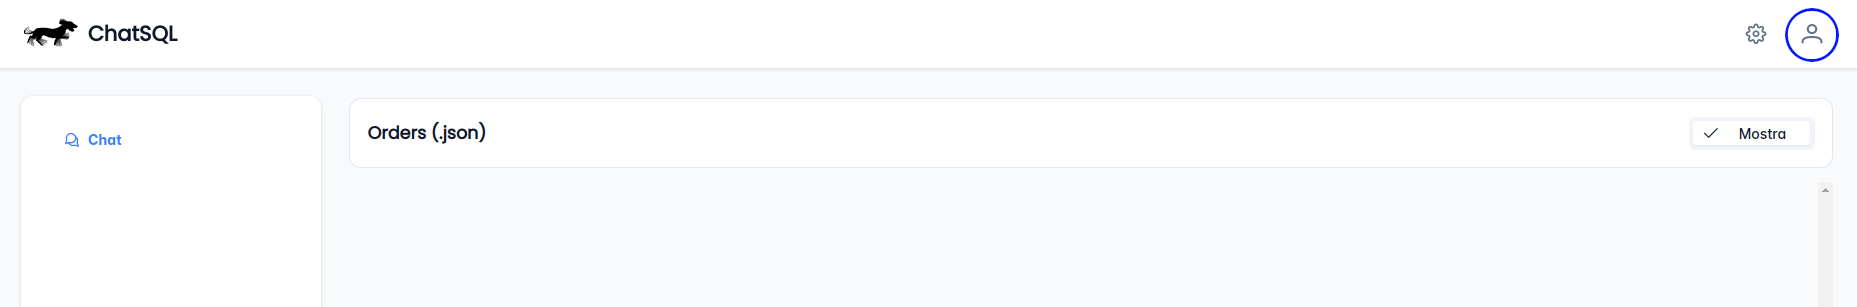
\includegraphics[width=1\textwidth]{assets/login_topbar.png}
  \caption{Topbar con menu di autenticazione}
\end{figure}
\begin{figure}[H]
  \centering
  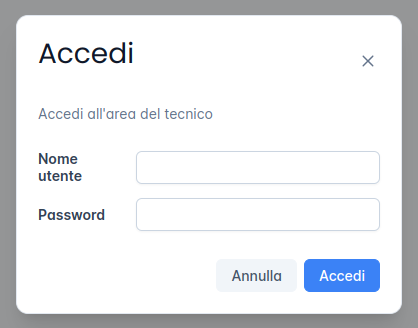
\includegraphics[width=0.50\textwidth]{assets/login_modal.png}
  \caption{Modale di login}
\end{figure}

\subsection{Gestione dizionari}
\begin{figure}[H]
  \centering
  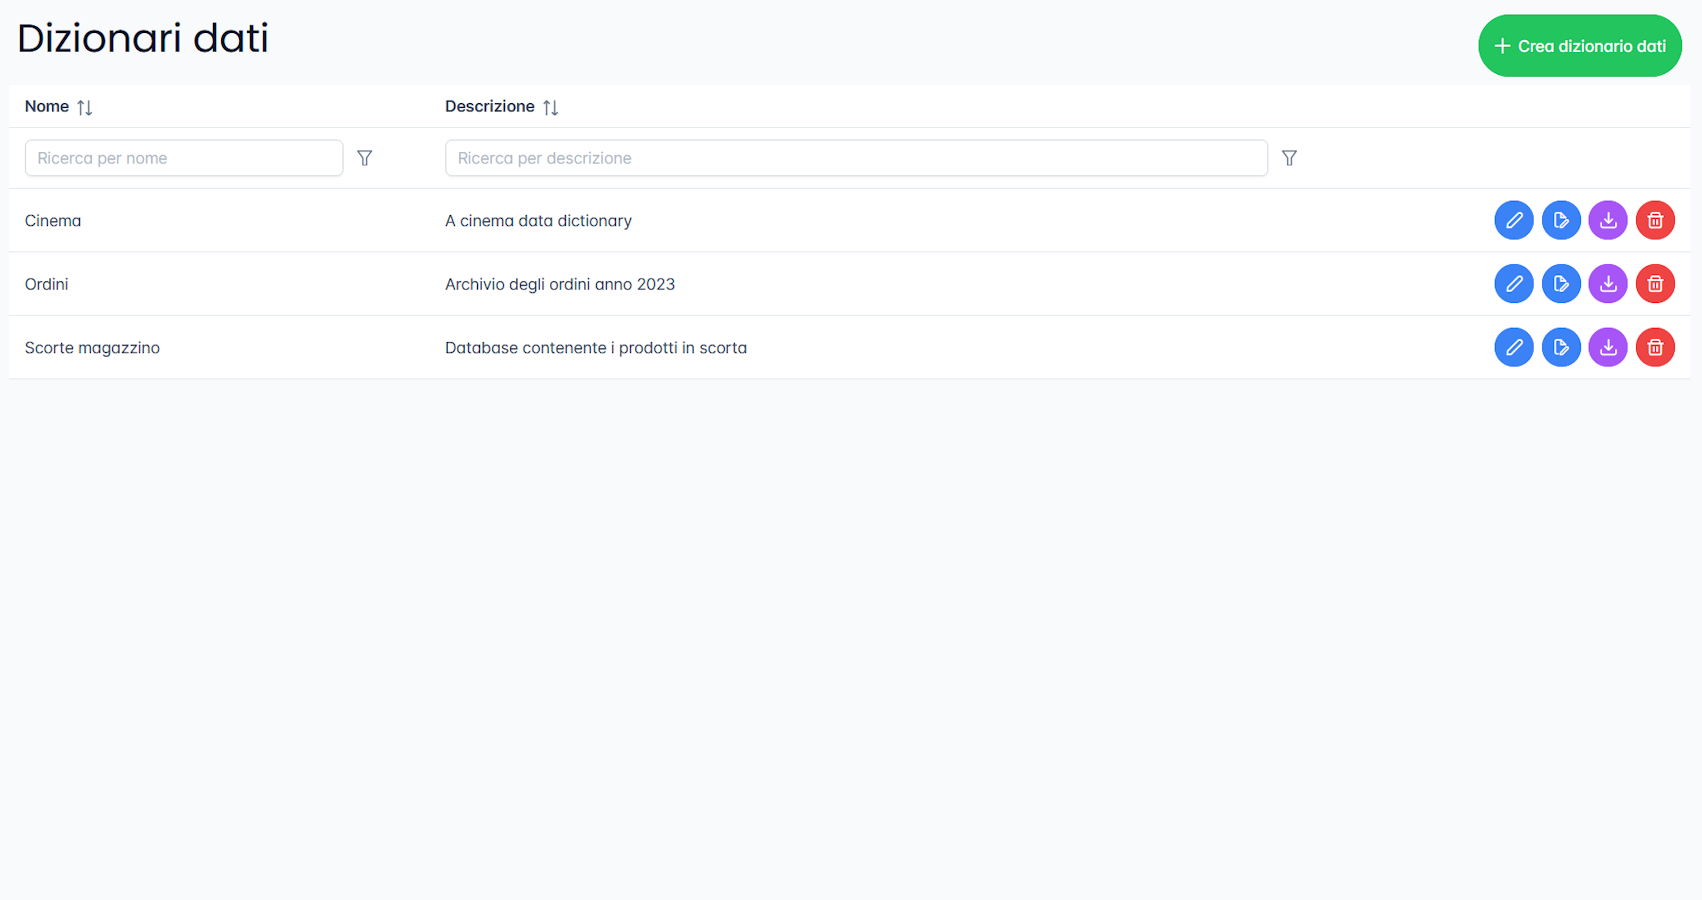
\includegraphics[width=1\textwidth]{assets/dd_list.png}
  \caption{Schermata di gestione dizionari dati}
\end{figure}
\par La schermata soprastante mostra la lista completa dei \glossario{dizionari dati} caricati nel sistema. Vengono fornite le funzionalità per operare su di essi.

\subsubsection{Aggiunta \glossario{dizionario dati}}
Cliccando sul pulsante "Crea dizionario dati" 
\includegraphics[height=1.2em]{assets/dd_create_button.png} si aprirà una modale dove sarà possibile inserire i parametri di un nuovo \glossario{dizionario dati}:
\begin{figure}[H]
  \centering
  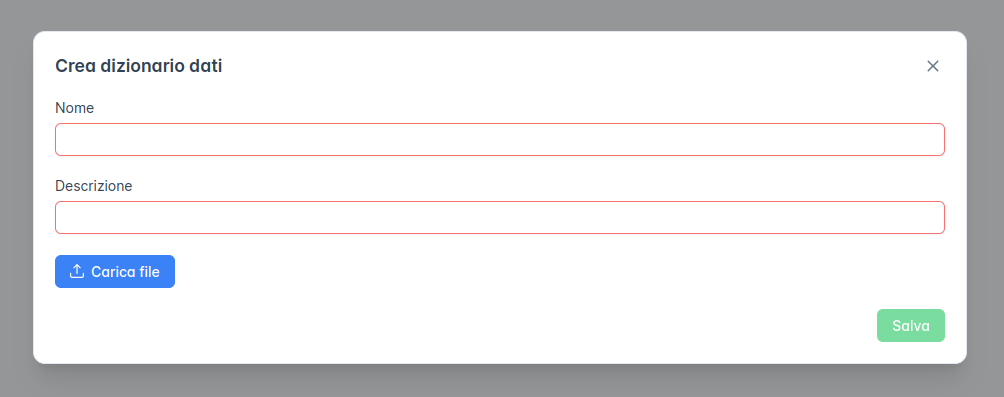
\includegraphics[width=0.5\textwidth]{assets/dd_modal_create.png}
  \caption{Modale di creazione dizionario dati}
\end{figure}
\begin{itemize}
  \item \textbf{Nome}: deve essere univoco rispetto agli altri dizionari dati;
  \item \textbf{Descrizione}: stringa testuale che descrive brevemente il dizionario dati;
  \item \textbf{File}: deve essere un file in formato JSON, di dimensione massima 1 MB e strutturato secondo il modello proposto.
\end{itemize}
Al salvataggio il dizionario verrà aggiunto alla lista.

\subsubsection{Aggiorna \glossario{dizionario dati}}
Cliccando sul pulsante di aggiornamento dei metadati 
\includegraphics[height=1.2em]{assets/dd_edit_metadata_button.png} si aprirà una modale dove sarà possibile modificare i parametri:
\begin{itemize}
  \item nome: deve essere univoco rispetto agli altri \glossario{dizionario dati};
  \item descrizione: stringa testuale che descrive brevemente il \glossario{dizionario dati};
\end{itemize}

\subsubsection{Aggiorna file \glossario{dizionario dati}}
Cliccando sul pulsante di modifica file del \glossario{dizionario dati} 
\includegraphics[height=1.2em]{assets/dd_edit_button.png} si aprirà una modale dove sarà possibile modificare il file del dizionari dati.

\subsubsection{Scarica file dizionario dati}
Cliccando sul pulsante di download 
\includegraphics[height=1.2em]{assets/dd_download_button.png} verrà scaricato il file del \glossario{dizionario dati} corrispondente in formato JSON.

\subsubsection{Elimina file dizionario dati}
Cliccando sul pulsante di cancellazione 
\includegraphics[height=1.2em]{assets/dd_delete_button.png} si aprirà una modale di conferma per l'eliminazione del \glossario{dizionario dati}.
\begin{figure}[H]
  \centering
  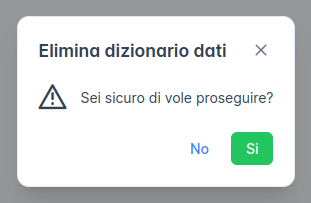
\includegraphics[width=0.5\textwidth]{assets/dd_confirm_delete.png}
  \caption{Modale di conferma eliminazione dizionario dati}
\end{figure}
In caso di conferma il dizionario verrà eliminato dalla lista.
